\section{Theorie}
\label{sec:Theorie}
Bei Schallwellen mit Frequenzen im Bereich von $\SI{20}{\kilo\hertz}$ bis $\SI{1}{\giga\hertz}$ handelt es sich um Ultraschall. Dieser wird genutzt um Informationen über nicht einsehbare
Strukturen oder Flüsse zu erhalten, ohne das Objekt, welches diese beinhaltet, zu beschädigen. Dies ist durch Aussenden eines Ultraschallpulses und Messen der Laufzeit und Frequenz der Reflexion
möglich. So kann zum Beispiel die Geschwindigkeit eines Teilchens unter Ausnutzung des Doppler-Effektes bestimmt werden. Dieses Verfahren wird Doppler-Sonographie genannt.
Der Doppler-Effekt tritt auf wenn sich die Quelle und/oder der Beobachter einer
Welle relativ zueinader bewegen. Falls Quelle oder Beobachter ruhen, verschiebt sich die Frequenz $\nu_0$ zu einer höheren Frequenz $\nu_h$, falls sich Quelle oder Beobachter auf den jeweils ruhenden
Beobachter oder Quelle zu bewegen. Bewegt sich einer vom anderen weg, wird die Frequenz zu einer niedrigeren Frequenz $\nu_n$ verschoben. Quantittativ wird dies durch
\begin{align}
  \nu_\text{h,n} &= \frac{\nu_0}{1\mp\frac{v}{c}}\\
  \intertext{für den ruhenden Beobachter, und}
  \nu_\text{h,n} &= \nu_0 \bigl(1\pm\frac{v}{c}\bigr)
\end{align}
für die ruhende Quelle, mit der jeweiligen Geschwindigkeit des bewegten Objektes $v$ und der Ausbreitungsgeschwindigkeit $c$, beschrieben.
\begin{figure}
  \centering
  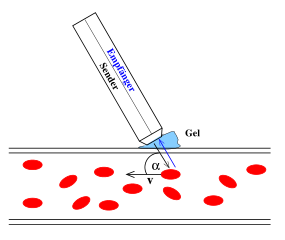
\includegraphics{images/dopplerfluss.png}
  \caption{Schematische Darstellung einer Doppler-Sonographie Messung an einem Blutgefäß.\cite{sample}}
  \label{fig:dopplerfluss}
\end{figure}
Wird nun ein Fluss in einem Gefäß mit einem Gemisch aus kleinen Festkörpern und Flüssigkeit, wie zum Beispiel Blut, untersucht, lässt sich mit den in Abbildung \ref{fig:dopplerfluss} dargestellten
geometrischen Zusammenhängen und unter Berücksichtigung der doppelten Doppler-Verschiebung durch das Reflektieren der Welle am bewegten Körper folgender Ausdruck für die Änderung der Frequenz
herleiten:
\begin{equation}
  \Delta\nu = 2 \nu_0\, \frac{v}{c} \cos(\alpha) .
  \label{eqn:deltanu}
\end{equation}
Zur genauen Untersuchung des Flusses in einem Rohr mittels Doppler-Sonographie werden Doppler-Prismen verwendet, welche bauartbedingt eine Untersuchung der Strömung aus verschiedenen Winkeln
unter gleichbleibenden Voraussetzungen erlauben.
\begin{figure}
  \centering
  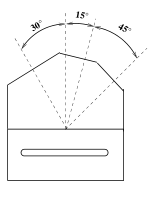
\includegraphics{images/prisma.png}
  \caption{Dopplerprisma.\cite{sample}}
  \label{fig:prisma}
\end{figure}
Dabei lässt sich für das in Abbildung \ref{fig:prisma} dargestellte Prisma folgender Zusammenhang zwischen Prismen- und Dopplerwinkel herleiten:
\begin{equation}
  \alpha = \SI{90}{\degree} - \arcsin\bigl(\sin(\theta)\cdot\frac{c_L}{c_P}\bigr) .
  \label{eqn:prisma}
\end{equation}
